
\documentclass[a4 paper,12pt]{article}
\usepackage[inner=2.0cm,outer=2.0cm,top=2.5cm,bottom=2.5cm]{geometry}
\usepackage{setspace}
\usepackage[rgb]{xcolor}
\usepackage{tabu}
\usepackage{pifont}
\usepackage{multirow}
\usepackage{longtable}
\usepackage{graphicx}
\usepackage{verbatim}
\usepackage{longtable}
\usepackage{subcaption}
\usepackage{fancyhdr}
\usepackage[colorlinks=true, urlcolor=blue, linkcolor=blue, citecolor=blue]{hyperref}
\usepackage{booktabs}
\usepackage{amsmath,amsfonts,amsthm,amssymb}
\usepackage{setspace}
\usepackage{listings}
\usepackage{fancyhdr}
\usepackage{lastpage}
\usepackage{tikz}
\usetikzlibrary{positioning, arrows.meta}
\usepackage{extramarks}
\usepackage{ctex,amsmath,amsfonts,amssymb,bm,hyperref,graphicx}
%\lstset{
	%	commentstyle=\color{red!50!green!50!blue!50},%代码块背景色为浅灰色
	%	rulesepcolor= \color{gray}, %代码块边框颜色
	%	breaklines=true,  %代码过长则换行
	%	numbers=left, %行号在左侧显示
	%	numberstyle= \small,%行号字体
	%	keywordstyle= \color{blue},%关键字颜色
	%	frame=shadowbox,%用方框框住代码块
	%	basicstyle=\ttfamily
	%}
\definecolor{dkgreen}{rgb}{0,0.6,0}
\definecolor{mauve}{rgb}{0.9,0.1,0.4}
\definecolor{ash}{rgb}{0.8,0.8,0.8}
\lstset{ 
	language=Octave,                % the language of the code
	basicstyle=\ttfamily,           % the size of the fonts that are used for the code
	numbers=left,                   % where to put the line-numbers
	numberstyle=\small\color{gray},  % the style that is used for the line-numbers
	stepnumber=1,                   % the step between two line-numbers. If it's 1, each line
	% will be numbered
	numbersep=5pt,                  % how far the line-numbers are from the code
	backgroundcolor=\color{ash},      % choose the background color. You must add \usepackage{color}
	rulesepcolor= \color{gray}, %代码块边框颜色
	showspaces=false,               % show spaces adding particular underscores
	showstringspaces=false,         % underline spaces within strings
	showtabs=false,                 % show tabs within strings adding particular underscores
	frame=single,                   % adds a frame around the code
	rulecolor=\color{black},        % if not set, the frame-color may be changed on line-breaks within not-black text (e.g. commens (green here))
	tabsize=2,                      % sets default tabsize to 2 spaces
	captionpos=b,                   % sets the caption-position to bottom
	breaklines=true,                % sets automatic line breaking
	breakatwhitespace=false,        % sets if automatic breaks should only happen at whitespace
	title=\lstname,                   % show the filename of files included with \lstinputlisting;
	% also try caption instead of title
	frame=shadowbox,%用方框框住代码块
	keywordstyle=\color{blue},          % keyword style
	commentstyle=\color{dkgreen},       % comment style
	stringstyle=\color{mauve},         % string literal style
	escapeinside={\%*}{*)},            % if you want to add LaTeX within your code
	morekeywords={*,...}               % if you want to add more keywords to the set
}
\usepackage{chngpage}
\usepackage{soul,color}
\usepackage{graphicx,float,wrapfig}
\newcommand{\homework}[3]{
	\pagestyle{myheadings}
	\thispagestyle{plain}
	\newpage
	\setcounter{page}{1}
	\noindent
	\begin{center}
		\framebox{
			\vbox{\vspace{2mm}
				\hbox to 6.28in { {\bf Microeconomics \hfill} {\hfill {\rm #2} {\rm #3}} }
				\vspace{4mm}
				\hbox to 6.28in { {\Large \hfill #1  \hfill} }
				\vspace{3mm}}
		}
	\end{center}
	\vspace*{4mm}
}
\newcommand\numberthis{\addtocounter{equation}{1}\tag{\theequation}}
\renewcommand\contentsname{Contents}
\begin{document}
	\homework{Homework05}{Group45}{吴熙楠}
	\tableofcontents
	\newpage
\section{Problem\quad 1}
\noindent
\textbf{Answer:}\\
(1)For NE:
\par $U_{1}=(a-b(q_{1}+q_{2}))q_{1}-cq_{1},U_{2}=(a-b(q_{1}+q_{2}))q_{2}-cq_{2}$
\par $\dfrac{dU_{1}}{dq_{1}}=0,\dfrac{dU_{2}}{dq_{2}}=0$ $\Rightarrow BR_{1}=q_{1}^{\star}=\dfrac{a-c-bq_{2}}{2b},BR_{2}=q_{2}^{\star}=\dfrac{a-c-bq_{1}}{2b}$
\par $BR_{1}=BR_{2}\Rightarrow q_{1}^{\star}=q_{2}^{\star}=\dfrac{a-c}{3b}$
\par So $q^{\star}=q_{1}^{\star}+q_{2}^{\star}=\dfrac{2(a-c)}{3b}$, total profit = $\dfrac{2(a-c)^{2}}{9b}$.
\\
(2)For monopoly:
\par Let's say company 1 is a monopoly, then we can get $q_{2}^{\star}=0$
\par So $\dfrac{dU_{1}}{dq_{1}}=0\Rightarrow a-2bq_{1}^{\star}=c\Rightarrow q_{1}^{\star}=\dfrac{a-c}{2b}$
\par So $q^{M}=\dfrac{a-c}{2b}$, total profit = $\dfrac{(a-c)^{2}}{4b}$.
\\
(3)For perfect competition:
\par $p(q_{1},q_{2})=MC=c\Rightarrow a-b(q_{1}^{\star}+q_{2}^{\star})=c$
\par So $q^{C}=q_{1}^{\star}+q_{2}^{\star}=\dfrac{a-c}{b}$, total profit = 0.
\section{Problem\quad 2}
\noindent
\textbf{Answer:}
\par (1)No. Because in this situation, $BR_{1}(L)=M,BR_{1}(R)=D,BR_{2}(U)=L$ or $R$,$BR_{2}(M)=R,BR_{2}(D)=L$
\par So we don't have any strictly dominated strategies for either player (in
pure strategies).
\par (2)No. Because player 2 only has 2 strategies, so we can only mix player 1's strategy. For player 1, if player 2 plays L, the worst responce is M and the best responce is D; if player 2 plays R, the worst responce is D and the best responce is M. So if we want to find the strictly dominated strategy, we can only mix M and D. We assume that the mixed strategy is (0,p,1-p). Then we must have that $3p>2,3(1-p)>2\Rightarrow p<\dfrac{1}{3}, p>\dfrac{2}{3}$. So we can't find this mixed strategy.
\par For player 2, if we want to have a strictly dominated strategy, the same as above, we should mix U and D. But if we use this strategy, this is not a strictly dominated strategy for player 1.
\par So there is not a strictly dominated strategy for either player.  
\par (3)Assume player 1 is mixing U, M and D with (0,p,1−p) and player 2's mixed strategy (q,1−q). Then we have these equations.
\par   $1-p=p,3q=3(1-q)\Rightarrow p=q=\dfrac{1}{2}$
\par So the mixed strategy is that $[(0,\dfrac{1}{2},\dfrac{1}{2}),(\dfrac{1}{2},\dfrac{1}{2})]$
\section{Problem\quad 3}
\noindent
\textbf{Answer:}
\par(a)Suppose (a,b) is the payoff, where a is the payoff of Li Lei and b is the payoff of Han Meimei. The payoff matrix is as following.
	\begin{figure}[H]
	\centering
	\hspace{2em}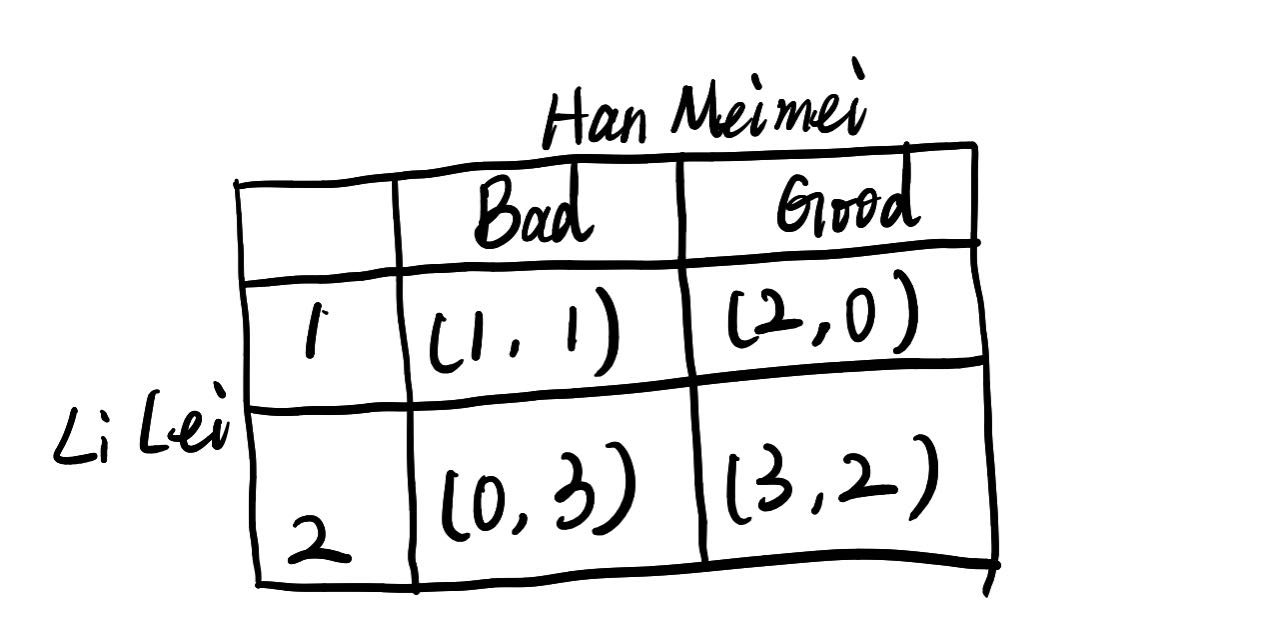
\includegraphics[width=.5\linewidth]{pic/1.jpg}
\end{figure}
\par From the payoff matrix,we know that, for Li Lei, $BR(Bad)=1,BR(Good)=2$. For Han Meimei, $BR(1)=Bad,BR(2)=Bad$.
\par So the NE is that Han Meimei makes bad hamburgers, and Li Lei buys one hanburg. It can be be expressed as (1,Bad).
\par (b)In the first selection, we know that (1,Bad) is the NE, so of course we will choose (1,Bad) in the first selection(Han Meimei makes bad hamburgers and Li Lei buys one hanburg).
\par But after the first selection, Li Lei gets 1 payoff and Han Meimei also gets 1 payoff. So we can think that the payoff matrix has no relative change(because two sides both add 1 payoff). So in the second selection, no matter what happens, Han Meimei makes bad hamburgers and Li Lei buys one hanburg(1,Bad). 
\par So the SPE is that in the first section, Han Meimei makes bad hamburgers, and Li Lei buys one hanburg(1,Bad); and in the second section, no matter what the result is in the first section, Han Meimei also makes bad hamburgers, and Li Lei also buys one hanburg(1,Bad).
\par (c)If Han Meimei always makes good hamburgers and Li Lei always buys two hanburgers. Then for Li Lei, the payoff is ($3+3\delta_{L}+3\delta_{L}^{2}+\cdots=\dfrac{3}{1-\delta_{L}}$). And for Han Meimei, the payoff is ($2+2\delta_{H}+2\delta_{H}^{2}+\cdots=\dfrac{2}{1-\delta_{H}}$).
\par If Li Lei violates the strategy, then the payoff will become ($2+\delta_{L}+\delta_{L}^{2}+\cdots=1+\dfrac{1}{1-\delta_{L}}$). And for Han Meimei, the payoff will become ($3+\delta_{H}+\delta_{H}^{2}+\cdots=2+\dfrac{1}{1-\delta_{H}}$).
\par So if we want to continue this strategy, we must have $\dfrac{3}{1-\delta_{L}}\ge 1+\dfrac{1}{1-\delta_{L}},\dfrac{2}{1-\delta_{H}}\ge 2+\dfrac{1}{1-\delta_{H}}$.
\par So from the inequalities above, we can get that $\dfrac{1}{2}\le \delta_{H}\le 1,0\le \delta_{L}\le 1$. 
\par So the minimum discount factor is that $\delta_{H}=\dfrac{1}{2}$ and $\delta_{L}=0$.
\end{document} 
